%%%%%%%%%%%%%%%%%%%%%%%%%%%%%%%%%%%%%%%%%%%%%%%%%%%%%%%%
\documentclass[12pt,a4paper]{article}% 文档格式
\usepackage{ctex,hyperref}% 输出汉字
\usepackage{times}% 英文使用Times New Roman
%%%%%%%%%%%%%%%%%%%%%%%%%%%%%%%%%%%%%%%%%%%%%%%%%%%%%%%%
\title{\fontsize{18pt}{27pt}\selectfont% 小四字号,1.5倍行距
	{\heiti% 黑体 
		计算流体力学期末作业}}% 题目
%%%%%%%%%%%%%%%%%%%%%%%%%%%%%%%%%%%%%%%%%%%%%%%%%%%%%%%%
\author{\fontsize{12pt}{18pt}\selectfont% 小四字号,1.5倍行距
	{\fangsong% 仿宋
		曹林博 \quad 2200011012}} % 标题栏脚注
%%%%%%%%%%%%%%%%%%%%%%%%%%%%%%%%%%%%%%%%%%%%%%%%%%%%%%%%
\date{}% 日期(这里避免生成日期)
%%%%%%%%%%%%%%%%%%%%%%%%%%%%%%%%%%%%%%%%%%%%%%%%%%%%%%%%
\usepackage{amsmath,amsfonts,amssymb}% 为公式输入创造条件的宏包
%%%%%%%%%%%%%%%%%%%%%%%%%%%%%%%%%%%%%%%%%%%%%%%%%%%%%%%%
\usepackage{graphicx}% 图片插入宏包
\usepackage{subfigure}% 并排子图
\usepackage{float}% 浮动环境,用于调整图片位置
\usepackage[export]{adjustbox}% 防止过宽的图片
%%%%%%%%%%%%%%%%%%%%%%%%%%%%%%%%%%%%%%%%%%%%%%%%%%%%%%%%
\usepackage{bibentry}
\usepackage{natbib}% 以上2个为参考文献宏包
%%%%%%%%%%%%%%%%%%%%%%%%%%%%%%%%%%%%%%%%%%%%%%%%%%%%%%%%
\usepackage{abstract}% 两栏文档,一栏摘要及关键字宏包
\renewcommand{\abstracttextfont}{\fangsong}% 摘要内容字体为仿宋
\renewcommand{\abstractname}{\textbf{摘\quad 要}}% 更改摘要二字的样式
%%%%%%%%%%%%%%%%%%%%%%%%%%%%%%%%%%%%%%%%%%%%%%%%%%%%%%%%
\usepackage{xcolor}% 字体颜色宏包
\newcommand{\red}[1]{\textcolor[rgb]{1.00,0.00,0.00}{#1}}
\newcommand{\blue}[1]{\textcolor[rgb]{0.00,0.00,1.00}{#1}}
\newcommand{\green}[1]{\textcolor[rgb]{0.00,1.00,0.00}{#1}}
\newcommand{\darkblue}[1]
{\textcolor[rgb]{0.00,0.00,0.50}{#1}}
\newcommand{\darkgreen}[1]
{\textcolor[rgb]{0.00,0.37,0.00}{#1}}
\newcommand{\darkred}[1]{\textcolor[rgb]{0.60,0.00,0.00}{#1}}
\newcommand{\brown}[1]{\textcolor[rgb]{0.50,0.30,0.00}{#1}}
\newcommand{\purple}[1]{\textcolor[rgb]{0.50,0.00,0.50}{#1}}% 为使用方便而编辑的新指令
%%%%%%%%%%%%%%%%%%%%%%%%%%%%%%%%%%%%%%%%%%%%%%%%%%%%%%%%
\usepackage{url}% 超链接
\usepackage{bm}% 加粗部分公式
\usepackage{multirow}
\usepackage{booktabs}
\usepackage{epstopdf}
\usepackage{epsfig}
\usepackage{longtable}% 长表格
\usepackage{supertabular}% 跨页表格
\usepackage{algorithm}
\usepackage{algorithmic}
\usepackage{changepage}% 换页
%%%%%%%%%%%%%%%%%%%%%%%%%%%%%%%%%%%%%%%%%%%%%%%%%%%%%%%%
\usepackage{enumerate}% 短编号
\usepackage{caption}% 设置标题
\captionsetup[figure]{name=\fontsize{10pt}{15pt}\selectfont Figure}% 设置图片编号头
\captionsetup[table]{name=\fontsize{10pt}{15pt}\selectfont Table}% 设置表格编号头
%%%%%%%%%%%%%%%%%%%%%%%%%%%%%%%%%%%%%%%%%%%%%%%%%%%%%%%%
\usepackage{indentfirst}% 中文首行缩进
\usepackage[left=2.50cm,right=2.50cm,top=2.80cm,bottom=2.50cm]{geometry}% 页边距设置
\renewcommand{\baselinestretch}{1.5}% 定义行间距(1.5)
%%%%%%%%%%%%%%%%%%%%%%%%%%%%%%%%%%%%%%%%%%%%%%%%%%%%%%%%
\usepackage{fancyhdr} %设置全文页眉、页脚的格式
\pagestyle{fancy}
\hypersetup{colorlinks=true,linkcolor=black}% 去除引用红框,改变颜色
%%%%%%%%%%%%%%%%%%%%%%%%%%%%%%%%%%%%%%%%%%%%%%%%%%%%%%%%



\begin{document}
	\maketitle
	
	\section{数理算法原理}
		\subsection{问题描述}
		针对Sod激波管问题,求解一维欧拉方程:
		\[
		 	\frac{\partial \mathbf{U}}{\partial t} + \frac{\partial \mathbf{f}(\mathbf{U})}{\partial x} = 0.
		\]
		其中:
		\[
		\mathbf{U} = 
		\begin{bmatrix}
		 	\rho \\
		 	\rho u \\
		 	E
		\end{bmatrix}, \quad
		\mathbf{f}(\mathbf{U}) = 
		\begin{bmatrix}
		 	\rho u \\
		 	\rho u^2 + p \\
		 	u(E + p)
		\end{bmatrix}, \quad
		E = \rho (e + \frac12 u^2) = \rho \left( C_v T + \frac{1}{2} u^2 \right)
		\]
		初始条件(在 $t=0$)为:
		\[
		\begin{cases}
		 	x < 0: & (\rho_L, u_L, p_L) = (1,\, 0,\, 1), \\
		 	x \ge 0: & (\rho_R, u_R, p_R) = (0.125,\, 0,\, 0.1).
		\end{cases}
		\]
		
		\subsection{Riemann精确解}
		该问题流程中,在连续部分满足控制方程:
		\[
		\left\{
		\begin{aligned}
		 	&\frac{\partial \rho}{\partial t} + \frac{\partial (\rho u)}{\partial x} = 0 \\
		 	&\frac{\partial (\rho u)}{\partial t} + \frac{\partial (\rho u^2 + p)}{\partial x} = 0 \\
		 	&\frac{\partial (E)}{\partial t} + \frac{\partial (E u + p u)}{\partial x} = 0
		\end{aligned}
		\right.
		\]
		其中,$E = \rho e = \rho (C_v T + \frac{1}{2} u^2)$.
		
		在间断部分满足间断条件$\mathbf{Rankine-Hugoniot}$关系式:
		\[
		\left\{
		\begin{aligned}
		 	& \rho_1(u_1 - Z) = \rho_2(u_2 - Z) \\
		 	& \rho_1 u_1(u_1 - Z) + p_1 = \rho_2 u_2(u_2 - Z) + p_2 \\
		 	& E_1(u_1 - Z) + u_1 p_1 = E_2(u_2 - Z) + u_2 p_2
		\end{aligned}
		\right.
		\]
		其中,$\mathbf{Z}$为激波运动速度。
		
		满足以上两个方程组的流场中可能产生三种波:
		\begin{enumerate}
		 	\item \textbf{激波:} 密度、速度、压力突变,满足$\mathbf{Rankine-Hugoniot}$关系式。
		 	\item \textbf{膨胀波:}等熵波,内部物理量连续光滑,头尾物理量连续但导数不连续.
		 	\item \textbf{接触间断:}两侧速度、压力相同,仅密度突变。
		\end{enumerate}
		
		因此流场组合共有以下五种:
		\begin{enumerate}
			\item 激波、接触间断、激波
			\item 膨胀波、接触间断、激波
			\item 激波、接触间断、膨胀波
			\item 膨胀波、接触间断、膨胀波
			\item 膨胀波、膨胀波
		\end{enumerate}
		
		经过对上述情况分析,我们将激波、膨胀波前后速度-压力的依赖关系写成统一的形式:
		\begin{enumerate}
		 	\item 左波(激波或膨胀波) $u^* = u_1 - f(p^*,p_1,\rho_1)$
		 	\item 右波(激波或膨胀波) $u^* = u_2 + f(p^*,p_2,\rho_2)$
		\end{enumerate}
		其中,$u^*,p^*$表示接触间断速度和压力,且有:
		\[
		f(p^*,p_i,\rho_i) = 
		\left\{
		\begin{aligned}
		 	& \frac{p^* - p_i}{\rho_i c_i[\frac{\gamma+1}{2\gamma} (\frac{p^*}{p_i}) + \frac{\gamma-1}{2\gamma}]^{1/2}},\quad p^*>p_i \\
		 	& \frac{2c_i}{\gamma-1}[(\frac{p^*}{p_i})^{\frac{\gamma-1}{2\gamma}} - 1],\quad p^*<p_i
		\end{aligned}
		\right.
		\]
		
		基于上述分析,我们可编写代码并求出Riemann精确解。
		 
		\subsection{NND+FVS+RK3方法}
		接下来,我们首先从NND格式(群速度方法)入手撰写激波捕捉格式,然后使用FVS类下Steger\_Warming通量分裂方法进行通量处理,最后使用Runge-Kutta方法推进时间积分。
		
		通过通量的分解,我们可以得到原欧拉方程组的NND格式为:
		\[
			(\frac{dU}{dt})_j = -\frac{1}{\Delta x}(H_{j+\frac12} - H_{j-\frac12})
		\]
		其中
		\begin{gather}
			H_{j+\frac12} = F^{+}_{j+\frac12L} + F^{-}_{j+\frac12R} \\
			F^{+}_{j+\frac12L} = F^+_j + \frac12 minmod(\Delta F^+_{j-1/2},\Delta F^+_{j+1/2}) \\
			F^-_{j+\frac12R} = F^-_{j+1} - \frac12 minmod(\Delta F^-_{j+1/2} , \Delta F^-_{j+3/2})
		\end{gather}
		
		而对于通量项,我们可由Steger\_Warming(FVS)通量分裂方法写为:
		\[
		\mathbf{f} = \frac{\rho}{2\gamma}
		\begin{bmatrix}
			2(\gamma - 1)\lambda_1 + \lambda_2 + \lambda_3 \\
			2(\gamma - 1)\lambda_1 u + \lambda_2 (u + c) + \lambda_3 (u - c) \\
			(\gamma - 1)\lambda_1 u^2 + \frac{(3 - \gamma)(\lambda_2 + \lambda_3)c^2}{2(\gamma - 1)} + \frac{\lambda_2 (u + c)^2}{2} + \frac{\lambda_3 (u - c)^2}{2}
		\end{bmatrix}
		\]
		其中,
		\[
		\begin{aligned}
			\text{当 } \lambda_i \geq 0,\quad & \lambda_i = \lambda_i,\quad \text{否则 } \lambda_i = 0,\quad \text{得到 } f^+ \\
			\text{当 } \lambda_i < 0,\quad & \lambda_i = \lambda_i,\quad \text{否则 } \lambda_i = 0,\quad \text{得到 } f^-
		\end{aligned}
		\]
		同时我们定义,
		\[
			minmod(x,y) = 
			\begin{cases}
				0, & xy \leq 0 \\
				sign(x)\min(|x|,|y|), & xy>0
			\end{cases}
		\]
		
		空间离散化后我们将式子记为:
		\[
			(\frac{dU}{dt})_j = -\frac{1}{\Delta x}(H_{j+\frac12} - H_{j-\frac12}) = f(u)
		\]
		根据Runge-Kutta方法,我们由如下推进时间计算公式:
		\[
		\left\{
			\begin{aligned}
				& u_1 = u^n + \frac13 \Delta t f(u^n) \\
				& u_2 = u^n + \frac21 \Delta t f(u_1) \\
				& u^{n+1} = \frac14 (u^n+3u_1) + \frac34 \Delta t f(u_2)
			\end{aligned}
		\right.
		\]
		
		基于上述推导,我们可求得Sod问题的近似解。
		
		\subsection{WENO+FDS+RK3方法}
		接下来,我们从HLLC格式(FDS)入手给出一种近似计算Riemann通量的方法,利用WENO格式构造U\_L,U\_R,使用Runge-Kutta方法推进时间求解。
		
		HLLC格式是基于HLL格式的改进格式,通过引入左行波、右行波和中间波,实现准确捕捉接触间断。首先我们估计左右波速:
		\[
		\begin{aligned}
			S_L &= min(u_L,u_R) - max(a_L,a_R) \\
			S_R &= max(u_L,u_R) + max(a_L,a_R)
		\end{aligned}
		\]
		通过求解自守恒的Rankine-Hugoniot条件,我们可得接触面速度:
		\[
			S_M = \frac{p_R - p_L + \rho_L u_L(S_L - u_L) - \rho_R u_R(S_R - u_R)}{\rho_L(S_L - u_L) - \rho_R(S_R - u_R)}
		\]
		以及求得中间状态压强:
		\[
			p^* = \frac12 (p_L+p_R)+\frac12[\rho_L(S_L-u_L)(S_M-u_L)+\rho_R(S_R-u_R)(S_M-u_R)]
		\]
		并定义用于加入压力项的方向向量:
		\[
			D = [0,1,S_M]
		\]
		按照如下公式我们可以计算通量:
		\[
			f_{j+\frac12} = 
			\left\{
				\begin{aligned}
					& f_L, \quad S_L \geq 0 \\
					& f_R, \quad S_R \leq 0 \\
					& \frac{S_M(S_L*U_L-f_L)+S_L*p^**D}{S_L - S_M}, \quad S_L\leq0,S_M\geq0 \\
					& \frac{S_M(S_R*U_R-f_R)+S_R*p^**D}{S_R - S_M}, \quad S_R\geq0,S_M\leq0 \\
				\end{aligned}
			\right.
		\]
		
		WENO作为高阶、非震荡格式的激波捕捉格式,通过加权不同基架系构造近似值。以构造$U_{i+\frac12}^+$为例,使用以下坐标系
		\[
			\begin{aligned}
				S_0 &= {U_{i-2},U_{i-1},U_{i}} \\
				S_1 &= {U_{i-1},U_i,U_{i+1}} \\
				S_2 &= {U_{i},U_{i+1},U_{i+2}}
			\end{aligned}
		\]
		对每组构造三阶近似:
		\[
			\begin{aligned}
				U_0 &= \frac13 U_{i-2} - \frac76 U_{i-1} + \frac{11}{6} U_{i} \\
				U_1 &= -\frac16 U_{i-1} + \frac56 U_{i} + \frac13 U_{i+1} \\
				U_2 &= \frac13 U_{i} + \frac56 U_{i+1} -\frac16 U_{i+2}
			\end{aligned}
		\]
		接下来按公式计算平滑指标:
		\[
			\begin{aligned}
				\beta_0 &= \frac{13}{12}(f_{i-2} - 2f_{i-1} + f_i)^2 + \frac{1}{4}(f_{i-2} - 4f_{i-1} + 3f_i)^2 \\
				\beta_1 &= \frac{13}{12}(f_{i-1} - 2f_i + f_{i+1})^2 + \frac{1}{4}(f_{i-1} - f_{i+1})^2 \\
				\beta_2 &= \frac{13}{12}(f_i - 2f_{i+1} + f_{i+2})^2 + \frac{1}{4}(3f_i - 4f_{i+1} + f_{i+2})^2
			\end{aligned}
		\]
		给定理想权重$d=[1,6,3]$,计算非线性权重为:
		\[
			\alpha_k = \frac{d_k}{(\epsilon + \beta_k)^2},\omega_k = \frac{\alpha_k}{\sum_j\alpha_j}
		\]
		从而最终构造$U$:
		\[
			U = \sum_{k=0}^{2} \omega_k U_k
		\]
		
		Runge-Kutta方法如之前所述,便不再赘述。由此我们求近似解。
		
		\subsection{TVD方法}
		接下来我们从TVD格式入手,构造限制器TVD格式,并使用高低通量计算公式计算边界通量,使用欧拉一阶向前算法推动时间步求解。
		
		考虑如下的离散方案:
		\[
			\frac{U_i^{n+1} - U_i^n}{\Delta t} = -\frac{1}{\Delta x}(F^n_{i+\frac12} - F^n_{i-\frac12})
		\]
		
		在计算单元边通量时,我们采取高低通量与限制器结合的格式:
		\[
			F^n_{i+\frac12} = F^{Low}_{i+\frac12} - \phi(r_i)(F^{Low}_{i+\frac12} - F^{High}_{i+\frac12})
		\]
		其中,给定计算公式:
		\[
			\begin{aligned}
				r_i &= \frac{U_i - U_{i-1}}{U_{i+1} - U_i} \\
				F^{Low}_{i+\frac12} &= \frac12(F_i + F_{i+1}) - \frac{\Delta x}{2\Delta t}(U_{i+1} - U_i) \\
				F^{High}_{i+\frac12} = \frac12(F_i + F_{i+1})
			\end{aligned}
		\]
		
		根据上述公式,我们可以推进计算近似解。
		
		
	\section{代码生成与调试}
		\subsection{Riemann精确解}
		我们在riemann.m文件中完成对Sod问题的Riemann精确解求解。算法流程分为以下三个步骤:
		\begin{enumerate}
			\item 根据公式$F(p^*) = f(p^*,p_1,\rho_1) + f(p^*,p_2,\rho_2) - u_1 + u_2$,利用牛顿迭代法求解中心区域压力值。
			\item 根据公式$u^* = \frac{1}{2}[u_1 + u_2 + f(p^*,p_2,\rho_2) - f(p^*,p_1,\rho_1)]$计算中心区域速度。并按前述公式确定两侧行波类型,计算中心区接触间断两侧的密度以及左右行波传播速度,及膨胀波区域内物理量。
			\item 将求解结果保存为三个视频,以可视化结果。
		\end{enumerate}
		
		\subsection{NND+FVS+RK3方法}
		我们在NND\_FVS\_RK3.m文件中完成对Sod问题的近似求解。算法流程大致分为以下几个步骤:
		\begin{enumerate}
			\item 计算声速和特征值。
			\item 根据Steger\_Warming公式计算守恒量通量项。
			\item 根据NND格式计算每个位置的通量及守恒量。
			\item 利用Runge-Kutta方法完成时间步推进。
			\item 将每次计算结果重画在画布上,从而方便展示结果动态变化过程,同时我们生成视频。
		\end{enumerate}
		
		\subsection{WENO+FDS+RK3方法}
		我们在WENO\_FDS\_RK3.m文件中完成对Sod问题的近似求解。算法流程大致分为以下几个步骤:
		\begin{enumerate}
			\item 根据WENO格式计算某位置处$U_L,U_R$。
			\item 根据HLLC格式完成通量及守恒量计算。
			\item 利用Runge-Kutta方法完成时间步推进。
			\item 将每次计算结果重画在画布上,从而方便展示结果动态变化过程,同时我们生成视频。
		\end{enumerate}
		
		\subsection{TVD方法}
		我们在TVD.m文件中完成对Sod问题的近似求解。算法流程大致分为以下几个步骤:
		\begin{enumerate}
			\item 根据上述公式计算响应的低通量和高通量,以及计算相应的$r_i$。
			\item 施加限制器,计算$F_{i+\frac12}$。
			\item 利用Euler向前计算方法完成时间步推进。(尝试过RK3方法,但是效果并不如Euler方法好)
			\item 将每次计算结果重画在画布上,从而方便展示结果动态变化过程,同时我们生成视频。
		\end{enumerate}

	\section{结果讨论}
		\subsection{Riemann精确解}
		\begin{figure}[H]
		\centering
		\begin{minipage}{0.83\textwidth}
			\centering
			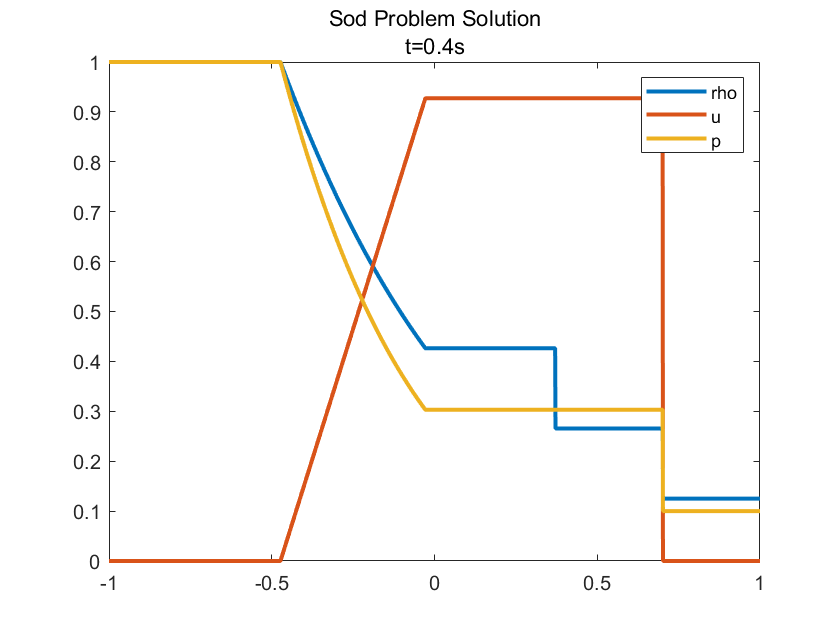
\includegraphics[width=\textwidth]{./fig/Riemann.png}
			\caption{\fontsize{10pt}{15pt}\selectfont Riemann精确解}
		\end{minipage}
		\end{figure}
		结果表明,该问题解为右行激波、左行膨胀波的情况,并分别展示了速度、压强和密度的演化。在密度结果图中我们也发现了接触间断的位置。

		\subsection{NND+FVS+RK3方法}
		\begin{figure}[H]
			\centering
			\begin{minipage}{0.83\textwidth}
				\centering
				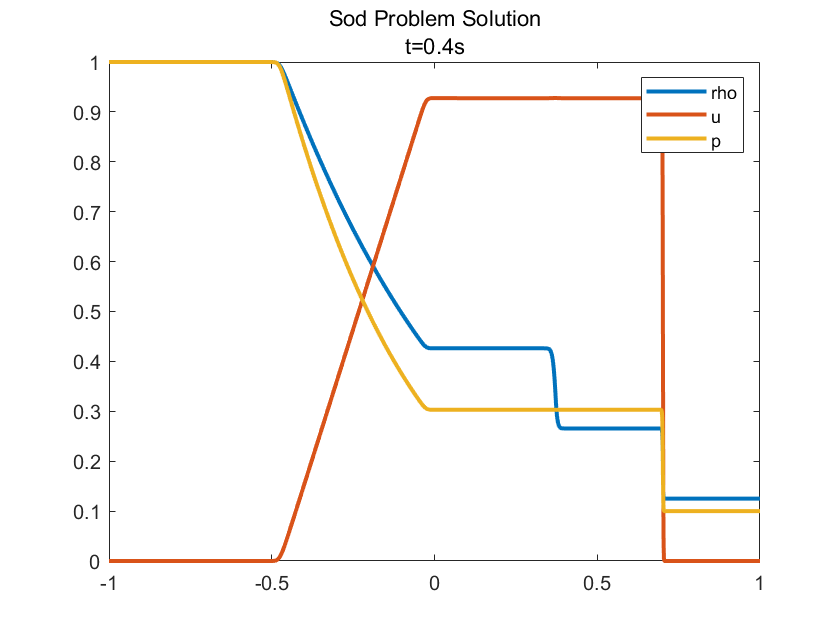
\includegraphics[width=\textwidth]{./fig/app1.png}
				\caption{\fontsize{10pt}{15pt}\selectfont NND+FVS+RK3方法近似解}
			\end{minipage}
		\end{figure}
		结果表明,该问题解与精确解相同。	
		
		\subsection{WENO+FDS+RK3方法}
		\begin{figure}[H]
			\centering
			\begin{minipage}{0.83\textwidth}
				\centering
				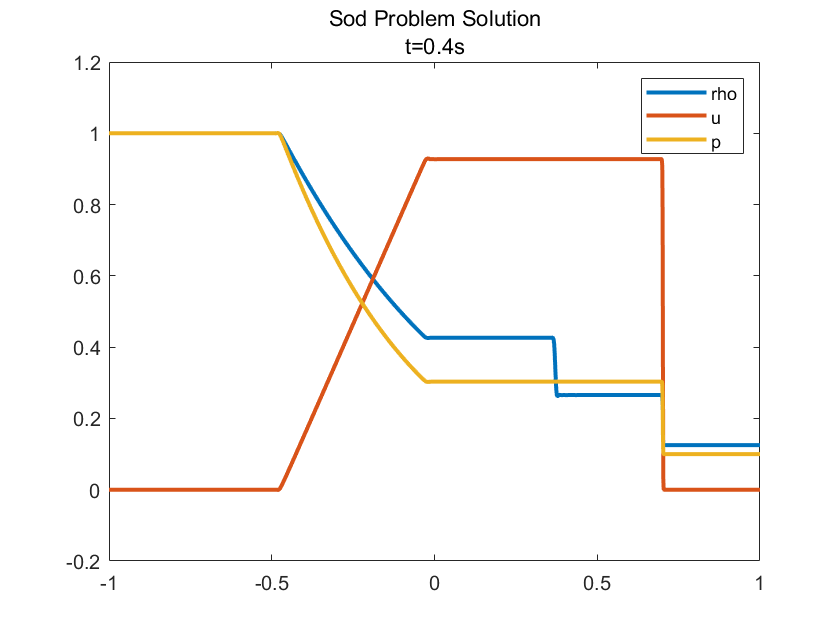
\includegraphics[width=\textwidth]{./fig/app2.png}
				\caption{\fontsize{10pt}{15pt}\selectfont WENO+FDS+RK3方法近似解}
			\end{minipage}
		\end{figure}
		结果表明,该问题解与精确解相同。	
		
		\subsection{TVD方法}
		\begin{figure}[H]
			\centering
			\begin{minipage}{0.83\textwidth}
				\centering
				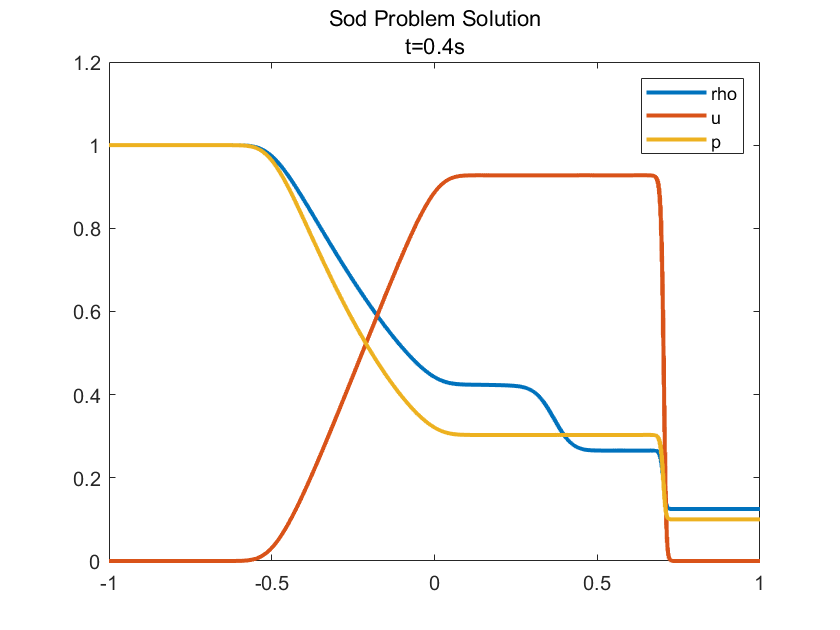
\includegraphics[width=\textwidth]{./fig/app3.png}
				\caption{\fontsize{10pt}{15pt}\selectfont TVD方法近似解}
			\end{minipage}
		\end{figure}
		结果表明,该问题解与精确解相同。	
			
	\section{附录}
		\begin{enumerate}
			\item 本题在作流场二次涡图时使用chatGPT帮助撰写绘图matlab代码。
			\item 本题代码文件设置较为清楚,且较为简单,故不使用git管理增加负担,无git管理记录。
		\end{enumerate}
	
\end{document}

